\chapter{Shortlist frameworks Augmented Reality}
\label{ch:shortlist}

In deze shortlist wordt de gekozen technologie uit de longlist, namelijk augmented reality, verder besproken.
Eerst volgt er een uitleg over wat de uiteindelijke applicatie moet bevatten.
Hierna volgt er een oplijsting van verschillende frameworks van augmented reality, deze frameworks zijn gekozen omdat ze elk iets bevatten wat hun uniek maakt. Per framework is er uitleg over wat het framework exact is, welke algoritmen deze gebruikt en aan welke requirements deze al dan niet voldoet. Aan de hand van deze krijgt elk framework dan een score krijgen die invloed heeft of dit framework wordt opgenomen in het experiment of niet.

\section{Uitleg AR Applicatie}\label{sec:arrequirements}
Volgende extra features zijn opgesteld eens de meest passende technologie bekend was. Deze functies maken gebruik van verschillende functionaliteiten die uniek zijn augmented reality waardoor het niet mogelijk was deze vroeger op te stellen.  Voor het opstellen van sommige van deze features is er inspiratie opgedaan van voorafgaande use cases.

De applicatie beschikt over de mogelijkheid om kunstwerken in te scannen en hierop digitale objecten te tonen. 
Om er voor te zorgen dat gebruikers niet te veel gebonden zijn aan de chronologie van het levensverhaal kunnen ze er ook voor kiezen om zonder rondleiding rond te lopen in het museum en op deze manier de kunstwerken te scannen.

Als extra moet er ook de mogelijkheid zijn om de virtuele objecten in de wereld te kunnen plaatsen, zonder het bijbehorend kunstwerk, door middel van plane detectie.

\section{Requirements}
Om de requirements van een applicatie op te schrijven zijn er verscheidene technieken. Voor deze use case worden de standaarden gebruikt van \textcite{Bradner1997}. Hierbij zijn er vijf verschillende soorten levels namelijk: MUST, MUST NOT, SHOULD, SHOULD NOT en MAY. Uit de bovenstaande uitleg over de applicatie en de uitleg in verband met teleprescence kunnen we volgende vereisten opstellen en ook nog enkele nice-to-haves toevoegen om de ervaring voor de gebruiker aangenamer te maken. Deze vereisten kunnen een positieve of negatieve invloed hebben op de score van het framework, de maximum score die een framework kan halen is 41.

\subsection{MUST}
Deze vereisten moet het framework sowieso ondersteunen en zullen dus veel harder doorwegen op de uiteindelijke score van het framework. Per MUST voorwaarde die voldaan is wordt de score met 5 verhoogt terwijl het ontbreken van een voorwaarde een negatieve invloed heeft van -5.
\begin{itemize}
    \item Ondersteuning van image herkenning
    \item Draaien op een groot aantal verschillende devices
    \item Klikken op het scherm linken aan een actie
    \item Tonen van informatie over het kunstwerk
    \item Ondersteunen verschillende 3d object formaten
\end{itemize} 

\subsection{MUST NOT}
Indien één van deze vereisten voorkomt bij het framework komt het framework niet meer in aanmerking komen om opgenomen te worden in het experiment.
\begin{itemize}
    \item Verplicht gebruik van specifieke hardware (bv. sensoren, depth camera)
    \item Verplicht gebruik van de meest recente versies van software waardoor sommige apparaten worden uitgesloten
\end{itemize} 

\subsection{SHOULD}
De SHOULD of RECOMMENDED vereisten zijn diegene waarbij het aangeraden is dat het framework ze ondersteunt maar zijn niet verplicht voor een basisimplementatie van de applicatie. Het hebben van deze vereisten verhoogt de score per vereiste met 3 maar heeft geen negatieve invloed  indien deze toch ontbreken.
\begin{itemize}
    \item Ondersteuning van plane detectie en het plaatsen van virtuele objecten hierop
    \item Ondersteuning van object herkenning
    \item Goede development documentatie
    \item Offline beschikbaar zijn
\end{itemize} 

\subsection{SHOULD NOT}
De opgelijste vereisten van deze categorie komen liefst niet voor in een framework maar het is niet zo erg indien ze toch zouden voorkomen zolang het framework genoeg andere MUST en SHOULD vereisten heeft. Het is hierdoor dat dit maar een kleine negatieve invloed heeft van -3.
\begin{itemize}
    \item Hevige drifting
\end{itemize} 

\subsection{MAY}
Deze vereisten zijn volledig optioneel en zullen niet zoveel invloed hebben op de score maar kunnen de ervaring van de gebruiker wel positief beïnvloeden. Omdat deze requirements optioneel zijn hebben ze maar een kleine positieve invloed op de score van +1.
\begin{itemize}
    \item Light estimation (aanpassen virtuele wereld indien licht in de echte wereld verandert)
    \item Ondersteuning van browser
     \item Virtuele buttons
     \item Images blijven tracken als ze bewegen
\end{itemize} 

\section{8th Wall}
Alhoewel het bedrijf achter 8th Wall zich de laatste tijd meer en meer hebben gefocust op 8th Wall Web heeft dit framework ook nog een tweede luik met 8th Wall XR. Het verschil tussen deze twee subframeworks is dat Web, zoals de naam het al duidelijk maakt, in een webbrowser draait. Echter zijn wel niet alle browsers ondersteund \autocite{8thWallWebReq}:
\begin{itemize}
    \item iOS
    \begin{itemize}
        \item Safari
    \end{itemize}
    \item Ondersteuning van browser
    \begin{itemize}
        \item Chrome
        \item Chrome varianten (Chromium browsers)
        \item Firefox
    \end{itemize}
\end{itemize} 


Hieronder volgt een kleine uitleg over beide subframeworks, echter is er wel gekozen om alleen van 8th Wall Web de requirements op te lijsten omdat de focus van het bedrijf vooral hierop ligt.

\subsection{8th Wall XR}
Met dit onderdeel van 8th Wall kunnen native augmented reality applicaties ontwikkeld worden voor Android en iOS. Dit framework maakt gebruik van de native technologieën (ARCore en ARKit) wanneer deze beschikbaar zijn. Bij devices die niet beschikken over deze technologie, omdat ze bijvoorbeeld verouderd zijn, zal 8th Wall zijn eigen \acrshort{slam} algoritme gebruiken.

\subsection{8th Wall Web}
Als enige framework in deze longlist bezit 8th Wall Web de mogelijkheid om in een browser te draaien. Dit zorgt ervoor dat de instapdrempel voor ontwikkeling redelijk laag ligt omdat vele developers al ervaring hebben met javasript en HTML.

Ook voor gebruikers kan een browser wel handig zijn omdat ze dan geen applicatie moeten downloaden eens ze in het museum zijn. Dit zorgt er natuurlijk wel voor dat er een goede netwerkinfrastructuur aanwezig moet zijn in het museum zodat de gebruiker de site kan gebruiken.

Op het tijdstip van het schrijven van deze shortlist bezat 8th Wall Web niet de mogelijkheid om afbeeldingen te herkennen. Recent heeft deze echter wel een update ontvangen waardoor dit framework nu wel deze mogelijkheid heeft. Omdat de rest van het onderzoek al was opgesteld, wordt deze functionaliteit niet opgenomen in de berekening van de score.

\subsection{Requirements}
8th Wall Web heeft een score van 13/41. Deze lage score komt omdat deze momenteel niet beschikt over image herkenning wat de belangrijkste feature is van de applicatie.
\begin{enumerate}
    \item MUST +5 score
    \begin{itemize}
        \item Draaien op een groot aantal verschillende devices (door native support van Android en iOS)
        \item Klikken op het scherm linken aan een actie 
        \item Ondersteunen verschillende 3d object formaten
    \end{itemize}
    \item MUST NOT, geen
    \item SHOULD +6 score
    \begin{itemize}
        \item Ondersteuning van plane detectie en het plaatsen van virtuele objecten hierop
        \item Goede development documentatie
    \end{itemize}
    \item SHOULD NOT, geen
    \item MAY +2 score
    \begin{itemize}
        \item Light estimation
        \item Ondersteuning van browser
    \end{itemize}
\end{enumerate}

\section{ARCore}
Het native AR framework voor Android, ontwikkeld door Google. Alhoewel dit framework speciaal gemaakt is voor Android biedt deze ook de mogelijkheid om apps te ontwikkelen voor iOS en zelfs voor een webbrowser \autocite{ARCoreOverview}. Omdat de webbrowser versie van ARCore alleen draait op Canary (de developer variant van Chrome) en ook hier nog eventjes zal blijven wordt deze niet verder besproken \autocite{ARCoreWeb}.

Voor het ontwikkelen van een applicatie met ARCore zijn er verschillende mogelijkheden. Er kan gekozen worden om puur native te gaan en gebruik te maken van de iOS of Android SDK, ook is er de optie om Unity of Unreal engine te gebruiken. Het voordeel hieraan is dat er veel keuze is in welke taal er geprogrammeerd kan worden. Wordt er Unreal of Unity gebruikt dan kunnen de ontwikkelde applicaties makkelijk worden omgezet om op iOS en Android te kunnen draaien. 

\subsection{Light Estimation}
ARCore heeft de mogelijkheid om variatie in licht te herkennen en hierdoor de lichtinval op de virtuele objecten aan te passen om zo meer het gevoel te geven dat ze daadwerkelijk in de wereld staan. Dit verhoogt dan weer het niveau van teleprescence \autocite{ARCoreConcepts}.

Niet alleen de lichtinval van de objecten kan worden aangepast, de virtuele objecten kunnen ook reageren op veranderingen in lichtniveau (zie figuur \ref{fig:arcoreLightEstimation}).

\begin{figure}
    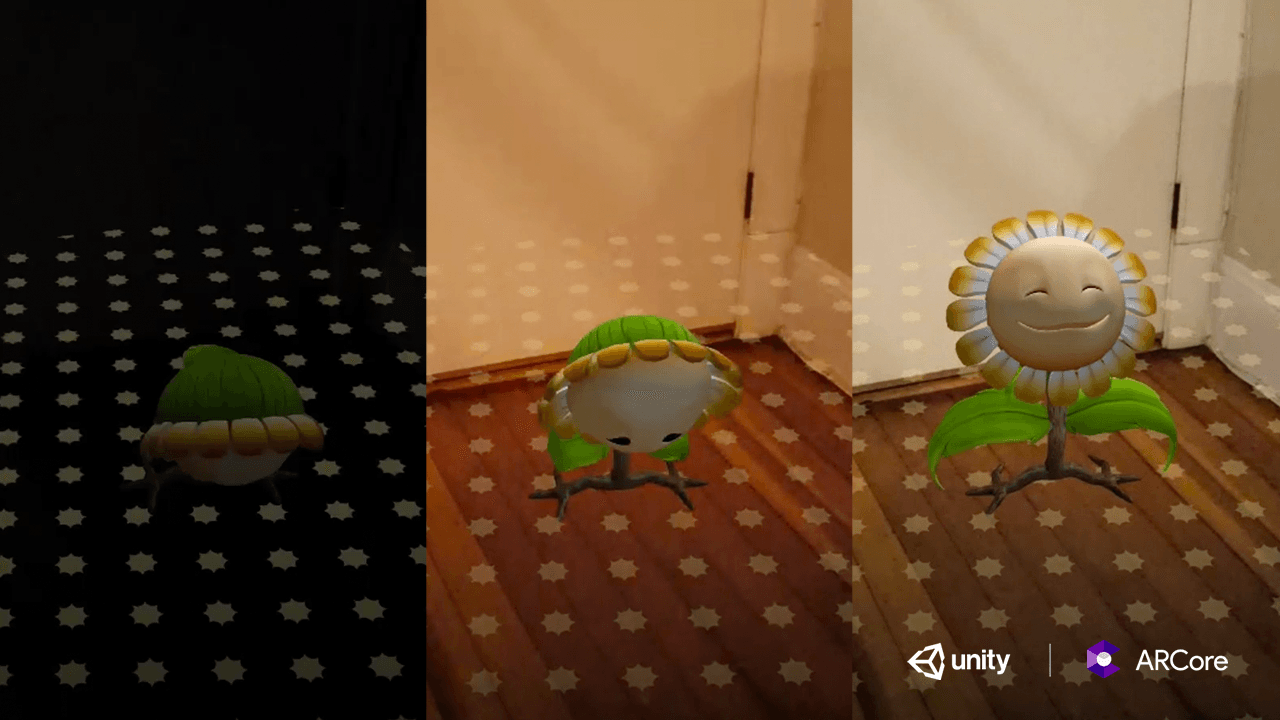
\includegraphics[width=\linewidth]{arcoreLightEstimation.png}
    \caption{Een virtueel object reageert anders afhankelijk van het lichtniveau}
    \label{fig:arcoreLightEstimation}
\end{figure}

\subsection{Cloud Anchors}
Meer en meer bedrijven kiezen ervoor om hun software in de cloud te hosten om zo zelf niet de infrastructuur te moeten voorzien. Het is dan logisch dat augmented reality ook deze mogelijkheid aanbied. Aan de hand van cloud anchors kan een ankerpunt in een ruimte worden gedeeld met andere gebruikers. 

Om een cloud anchor aan te maken moet de gewenste ruimte eerst gemapped zijn en hierin een ankerpunt zijn gecreëerd. De applicatie zal dan de relatieve positie van dit punt naar verhouding van nabijgelegen feature points versturen naar de Google servers die deze data dan zal hosten. 

Het hosten van deze data gebeurt door een Firebase databank die aan elk punt een id geeft, eens een ankerpunt gehost is zal de server een roomcode terugsturen waarmee andere gebruikers het anker kunnen zien. Omdat een kamer soms meerdere ankerpunten heeft kan het ook soms zijn dat er meerdere punten aan één roomcode worden gelinkt \autocite{ARCoreCloudAnchors}.

% TODO TRANSLATE relative => De relatieve positie van dit punt naar verhouding van... ? ASK!
\subsection{Requirements}
ARCore heeft een score van 36/41 door vooral goed te scoren op de MUST voorwaarden. Alhoewel ARCore misschien niet beschikt over een uitgebreide implementatie van deze voorwaarden is het vooral belangrijk dat ze aanwezig zijn binnen het framework.
\begin{enumerate}
    \item MUST +25 score
    \begin{itemize}
       \item Ondersteuning van image herkenning
       \item Draaien op een groot aantal verschillende devices (door native support van Android en iOS)
       \item Klikken op het scherm linken aan een actie 
       \item Tonen van informatie over het kunstwerk
       \item Ondersteunen verschillende 3d object formaten
    \end{itemize}
    \item MUST NOT, geen
    \item SHOULD +9 score
    \begin{itemize}
    \item Ondersteuning van plane detectie en het plaatsen van virtuele objecten hierop
    \item Goede development documentatie
    \item Offline beschikbaar zijn
    \end{itemize}
    \item SHOULD NOT, geen
    \item MAY +2 score
    \begin{itemize}
        \item Light estimation
        \item Images blijven tracking
    \end{itemize}
\end{enumerate}

\section{ARKit}
ARKit is de native technologie voor iOS, in tegenstelling tot ARCore kan men met dit framework alleen maar iOS applicaties ontwikkelen.

De ontwikkeling van ARKit applicaties kan gebeuren via XCode (de IDE van Apple), Unity of Unreal. XCode zal gebruik maken van Swift of Objective C terwijl Unity en Unreal hun programmeertaal gebruiken (C\# en C++ respectievelijk).
% TODO CONTENT Extra info

\subsection{Persistent Mapping}
Sinds ARKit 2.0 is er de mogelijkheid om persistent mapping in ARKit applicaties te implementeren. Met dit kan een gemapte ruimte worden opgeslagen zodat de mapping tussen sessies opgeslagen blijft.
Om bij een volgende sessie de mapping op te halen moet de camera van de smartphone terug worden geplaatst naar de locatie waar de mapping was opgeslagen. Eens deze volledig geladen is kunnen ook de ankerpunten worden teruggezet inclusief hun virtuele objecten \autocite{ARKitPersistent}.

\subsection{Multiuser Experience}
Dit is een uitbreiding van persistent mapping waarbij mapping data tussen apparaten kan worden gedeeld. Het eerste apparaat moet de ruimte scannen en kan deze data dan doorsturen naar andere apparaten. Wanneer een virtueel object wordt geplaatst in de ruimte zal deze worden getoond bij alle apparaten.

Om de communicatie tussen de devices te regelen wordt er gebruikgemaakt van peer-to-peer networking. Dit betekent dat, in tegenstelling met ARCore, er geen server nodig is om ankerpunten te delen. Het grote nadeel aan deze functionaliteit is dat de applicatie zich (zonder extra configuratie) gaat verbinden met de eerst gevonden sessie. Indien dit niet correct geconfigureerd is, kan dit wel voor problemen zorgen in plaatsen waar er veel sessies tegelijk zouden zijn zoals in musea.

Hoewel er geen server nodig is kan het soms wel handig zijn dat een apparaat als server handelt, indien dit gewenst is kan dit worden ingesteld.

Nog een groot verschil met ARCore is dat bij ARCore alleen de locatie en feature points van de ankerpunten worden teruggestuurd terwijl ARKit de hele mapping data verstuurt. Het versturen van deze data kan heel wat bandbreedte opnemen dus kunnen er problemen optreden indien er veel apparaten zijn die met dezelfde sessie willen verbinden \autocite{ARKitMultiuser}.

\subsection{Requirements}
ARKit heeft een score 29/41 omdat dit framework alleen maar draait op iOS devices. Dit zorgt ervoor dat de requirement 'Draaien op een groot aantal devices' geschonden is waardoor de score met 5 vermindert wordt.
\begin{enumerate}
    \item MUST +15 score
    \begin{itemize}
        \item Ondersteuning van image herkenning
        \item Klikken op het scherm linken aan een actie 
        \item Tonen van informatie over het kunstwerk
        \item Ondersteunen verschillende 3d object formaten
        \item Ontbreken support groot aantal devices, score -5
    \end{itemize}
    \item MUST NOT, geen
    \item SHOULD +12 score
    \begin{itemize}
        \item Ondersteuning van plane detectie en het plaatsen van virtuele objecten hierop
        \item Ondersteuning van object herkenning (alleen bij ARKit 2.0)
        \item Goede development documentatie
        \item Offline beschikbaar zijn
    \end{itemize}
    \item SHOULD NOT, geen
    \item MAY +2 score
    \begin{itemize}
        \item Light estimation
        \item Images blijven tracking
    \end{itemize}
\end{enumerate}

\section{Vuforia}
Net zoals 8th Wall en ARCore biedt Vuforia de mogelijkheid om native applicaties te ontwikkelen voor Android en iOS. Vele andere frameworks ondersteunen ook het herkennen van images en sommige zelfs objecten maar geen enkel ander framework focust zich hier evenveel op als Vuforia.  

Ontwikkeling van Vuforia applicaties kan gebeuren in de native development omgevingen van Android, iOS en UWP door gebruik te maken van passende SDK. Ook is er de mogelijkheid om applicaties te ontwikkelen in Unity, deze kunnen dan draaien op alle bovenstaande native technologieën.

\subsection{Fusion}
Het unieke aan Vuforia is de manier waarop deze \acrshort{slam} implementeert. Vuforia zal zoveel mogelijk proberen gebruik te maken van de native mapping algoritmen (ARKit, ARCore en MR). Hierdoor kan deze gebruikmaken van alle features die deze native technologieën bevatten alsook nog zijn eigen functionaliteiten hieraan toevoegen. Op deze manier ondersteunt Vuforia direct alle apparaten die gebruikmaken van ARKit, ARCore en MR. Voor apparaten die niet ondersteunt zijn door deze frameworks is er VISLAM en \acrshort{slam}. Hierdoor is er ook ondersteuning voor oudere apparaten die ARKit of ARCore niet ondersteunen \autocite{VuforiaFusion}.
\begin{figure}
    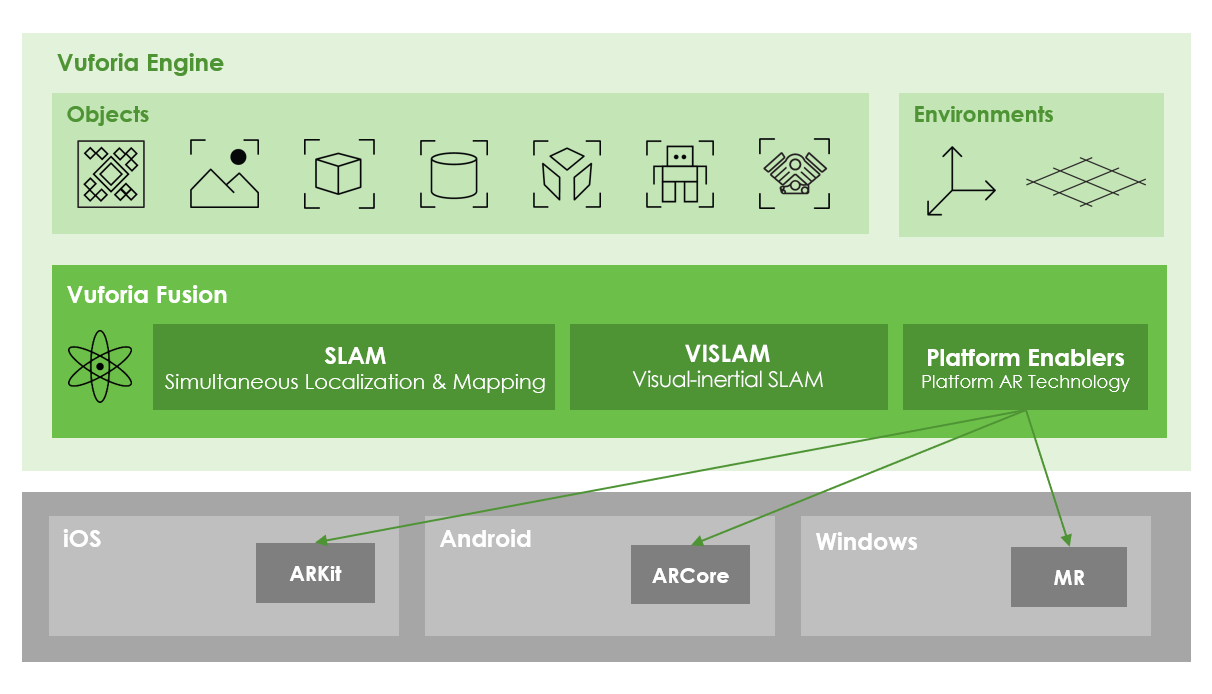
\includegraphics[width=\linewidth]{vuforiaFusion.png}
    \caption{Vuforia Fusion}
    \label{fig:vuforiaFusion}
\end{figure}

\subsection{Cloud Recognition}
Om afbeeldingen te herkennen is er een image target database nodig. Omdat deze database soms redelijk groot kan worden bij applicaties die veel afbeeldingen bevatten is het aangeraden om hierbij gebruik te maken van een online database om een goede performance te garanderen \autocite{VuforiaCloudReco}. 

Er is ook de mogelijkheid om metadata te linken aan de images in de databank. Hierdoor kan de applicatie weten wat hij exact moet tonen in de virtuele wereld. Het is mogelijk om verschillende soorten data hieraan te linken waaronder: JSON, URLS of zelfs een volledig 3d object (zolang deze onder de geheugengrootte zit van 2MB) \autocite{VuforiaCloudReco}.

\subsection{Targets}
Vuforia bied vijf soorten herkenning aan, deze worden hieronder kort uitgelegd wat ze exact doen en hoe ze werken.

\begin{itemize}
    \item Image Targets: gewone afbeeldingen
    \item Model Targets: het herkennen van 3d objecten en deze veranderen in een virtueel object
    \item Multi Targets: meerdere afbeeldingen herkennen en deze samenvoegen
    \item VuMarks: soort van custom QR Codes zie figuur \ref{fig:vumarks}
    \item Cylinder Targets: afbeelding herkennen op een cylinder vorm
\end{itemize} 

\begin{figure}
    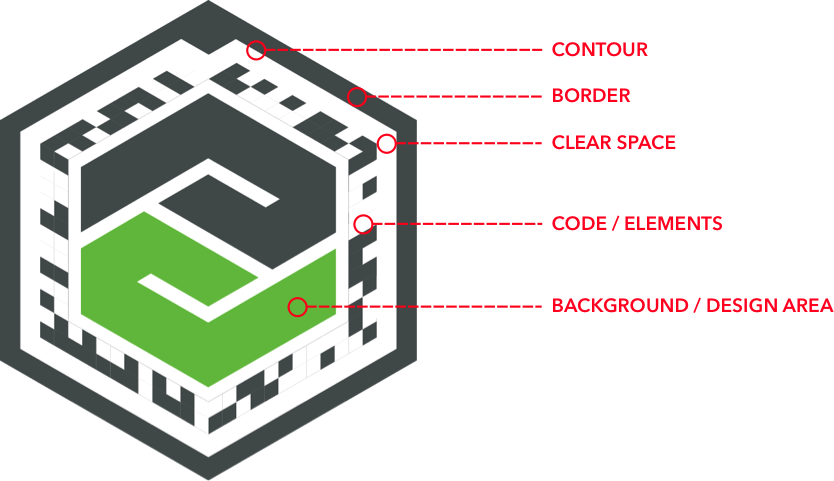
\includegraphics[width=\linewidth]{vumarks.png}
    \caption{Opbouw van een VuMark, de developer kan kiezen hoe deze eruit ziet zolang de contour (vorm), border en clear space aanwezig zijn. Vuforia gebruikt de code elements om data te encoderen}
    \label{fig:vumarks}
\end{figure}

\subsection{Requirements}
Vuforia heeft een score 37/41 door zijn grote focus op de benodige requirements alsook de nice-to-haves. Door zijn multiplatform (Android en ioS) support in combinatie met eigen features krijgt deze een hoge score. Echter bij het testen van dit framework is het wel gebleken dat er zich hevige drifting voordoet wanneer de plane detection functie wordt gebruikt. Dit voorval heeft een kleine negatieve invloed op de score van Vuforia.
\begin{enumerate}
    \item MUST +25 score
    \begin{itemize}
        \item Ondersteuning van image herkenning
        \item Draaien op een groot aantal verschillende devices (door native support van Android en iOS)
        \item Klikken op het scherm linken aan een actie 
        \item Tonen van informatie over het kunstwerk
        \item Ondersteunen verschillende 3d object formaten
    \end{itemize}
    \item MUST NOT, geen
    \item SHOULD +12 score
    \begin{itemize}
        \item Ondersteuning van plane detectie en het plaatsen van virtuele objecten hierop
        \item Ondersteuning van object herkenning
        \item Goede development documentatie
        \item Offline beschikbaar zijn
    \end{itemize}
    \item SHOULD NOT -3 score
    \begin{itemize}
        \item Hevige drifting
    \end{itemize}
    \item MAY +3 score
    \begin{itemize}
        \item Light estimation (momenteel alleen bij ARKit)
        \item Virtuele buttons
        \item Images blijven tracking
    \end{itemize}
\end{enumerate}

\section{Conclusie Shortlist}
Uit deze shortlist blijkt dat ARCore en Vuforia de twee hoogste scorende frameworks zijn. Dit betekent echter niet dat deze de beste frameworks zijn, maar eerder dat deze minstens over alle nodige basisfunctionaliteiten van de applicatie beschikken. Deze twee frameworks worden nu verder met elkaar vergeleken in het experiment waarbij zal worden getest hoe goed zijn deze functionaliteiten implementeren alsook hoe goed hun performance is.